\documentclass[preprint,11pt]{elsarticle}

\usepackage[top=2.2cm,bottom=2.4cm,left=2.4cm,right=2.4cm,headheight=15pt,headsep=0.7cm,footskip=1.1cm]{geometry}

\usepackage[T1]{fontenc}
\usepackage[utf8]{inputenc}
\usepackage{graphicx}
\usepackage{amsmath,amsthm}
\usepackage{newtxtext,newtxmath}% Times + math (provee simbolos amssymb)
\usepackage{microtype}
\usepackage{booktabs}
\usepackage{float}
\floatplacement{table}{H}   % todo float fica exatamente onde está no fonte
\floatplacement{figure}{H}
\usepackage{enumitem}
\setlist{nosep,leftmargin=*}
\usepackage{url}
\usepackage[hidelinks]{hyperref}

%% ---- Teoremas --------------------------------------------------------
\newtheorem{theorem}{Theorem}[section]
\newtheorem{lemma}[theorem]{Lemma}
\newtheorem{proposition}[theorem]{Proposition}
\newtheorem{corollary}[theorem]{Corollary}
\theoremstyle{definition}
\newtheorem{definition}[theorem]{Definition}
\theoremstyle{remark}
\newtheorem{remark}[theorem]{Remark}

%% ---- Notacao ---------------------------------------------------------
\newcommand{\cA}{\mathcal{A}}
\newcommand{\cB}{\mathcal{B}}
\newcommand{\cP}{\mathcal{P}}
\newcommand{\cL}{\mathcal{L}}
\newcommand{\C}{\cite{Campbell2026}}
\numberwithin{equation}{section}

\setlength{\emergencystretch}{3em}
\setlength{\abovedisplayskip}{6pt plus 2pt minus 2pt}
\setlength{\belowdisplayskip}{6pt plus 2pt minus 2pt}
\setlength{\abovedisplayshortskip}{3pt plus 1pt}
\setlength{\belowdisplayshortskip}{3pt plus 1pt}
\renewcommand{\topfraction}{0.9}
\renewcommand{\bottomfraction}{0.9}
\renewcommand{\textfraction}{0.1}
\renewcommand{\floatpagefraction}{0.8}

\journal{Journal of Number Theory}

\begin{document}

\begin{frontmatter}

\title{Goldbach-type sums \texorpdfstring{$a+b=N$}{a+b=N} with \texorpdfstring{$\Omega(ab)\le 32$}{Omega(ab) <= 32}}

\author{Giovane de Morais}
\ead{giovanedms@gmail.com}
\affiliation{organization={Centro de Compet\^encia em Manufatura (CCM), Graduate Program in Aeronautical and Mechanical Engineering, Instituto Tecnol\'ogico de Aeron\'autica (ITA)},
            city={S\~ao Jos\'e dos Campos},
            state={SP},
            country={Brazil}}

\begin{abstract}
We prove that every integer $N\ge 2$ can be written as $N=a+b$ with
positive integers $a,b$ such that $\Omega(ab)\le 32$, where $\Omega$
counts prime factors with multiplicity. This improves the bound
$\Omega(ab)\le33$ of Campbell. The argument stays inside Campbell's
framework, the explicit Friedlander--Iwaniec lower-bound sieve applied to
the products $n(N-n)$. Three elementary reductions lead to a sieve
estimate at a level depending on the parity of $N$; the hard case is odd
$N$, with $z=(N^2/8)^{1/32}$. We close it with a per-interval dimension constant, per-interval sieve parameters
and pre-sieving by both $3$ and $5$. The intermediate range is certified in ball arithmetic over
$117\,415$ intervals, and the large range by a monotonicity argument; the
even case is certified in the same way. For completeness we include a
self-contained proof of the explicit Friedlander--Iwaniec lower bound with
the dimension condition imposed only at the sifting level.
\end{abstract}

\begin{keyword}
Almost primes \sep Goldbach-type theorems \sep sieve methods \sep
explicit bounds \sep ball arithmetic
\MSC[2020] 11P32 \sep 11N36 \sep 11Y35
\end{keyword}

\end{frontmatter}

%% =====================================================================
\section{Introduction}\label{sec:intro}
%% =====================================================================

Let $\Omega(n)$ denote the number of prime factors of $n$ counted with
multiplicity. Chen's theorem~\cite{Chen1973} represents every sufficiently
large even integer as a prime plus an integer with at most two prime
factors, and R\'enyi's theorem~\cite{Renyi1948} gives a uniform bound for
all even $N\ge4$ with an unspecified constant. Johnston and
Starichkova~\cite{JS2025} made R\'enyi's theorem explicit: every even
$N\ge 4$ is $p+r$ with $p$ prime and $\Omega(r)\le 395$, and
$\Omega(r)\le 31$ under the generalised Riemann hypothesis. Their proof
uses the explicit linear sieve of Bordignon, Johnston and
Starichkova~\cite{BJS2025}.

Relaxing the condition that one summand be prime, one asks for $N=a+b$
with $\Omega(ab)$ small. Dudek and Dunn~\cite{DudekDunn} proved
$\Omega(ab)\le 40$ for every $N\ge2$, applying the explicit
Friedlander--Iwaniec $\Lambda^-\Lambda^2$ lower-bound sieve~\cite{FI2010}.
In their setting the extremal case $w=3$ of the dimension condition forces
the constant $K=3$. Campbell~\C{} removed this case by pre-sieving at the
prime $3$ and obtained $\Omega(ab)\le 33$. He also wrote that
$\Omega(ab)\le 32$ ``appears to be within reach'' and listed four possible
refinements: $K$ computed per interval; $s$ and $\delta$ optimised per
interval; pre-sieving by $3$ and $5$; sharper constants~\cite[\S6]{Campbell2026}.

\begin{theorem}\label{thm:main}
Every integer $N\ge 2$ can be written as $N=a+b$ with
$a,b$ positive integers and
\[
  \Omega(ab)\le 32 .
\]
\end{theorem}

Campbell applies Theorem~\ref{thm:FI} with the dimension condition read at
the sifting level only (``for each value of $z$ under
consideration''~\cite[(2.1)]{Campbell2026}); the global reading, over all
pairs $2\le w<z'$, would force $K\ge2$, which is incompatible with his
constant $K=1.146$ (Remark~\ref{rem:global}). For completeness we prove
that this local reading suffices (Theorem~\ref{thm:local},
Appendix~\ref{app:sieve}). We do not claim novelty for this statement: the
proof is Selberg's $\Lambda^-\Lambda^2$ argument as presented by
Blight~\cite{Blight2010}, the dimension condition enters only through a
Rankin bound at the level $z$, and the statement may well be implicit
in~\cite[\S7]{FI2010}; we include it so that the paper does not depend on
how the condition is read.

\paragraph{Where $33$ comes from}
The bound $33$ comes only from odd $N$. With $z=N^{1/r}$ and $a_n<N^2$,
\cite[Lemma~5.2]{Campbell2026} gives $\Omega(ab)<2r$ for even $N$ and
$\Omega(ab)<2r+1$ for odd $N$; with $r=16.5$ this is $\le32$ and $\le33$
respectively. Three elementary observations
(Section~\ref{sec:reductions}) reduce the problem to an estimate at a
level depending on the parity of $N$: for even $N$ the sifting level
$z=(N^2/4)^{1/33}$ suffices, and this case has a wide margin; the prime-gap lemma \cite[Lemma~5.1]{Campbell2026}
holds under $1854m<2^{M-1}$ instead of $1854m\le2^{M-2}$, which covers
$N\le N_0$ with $M=32$; and for odd $N$ one has $a_n\le(N^2-1)/8$, so the
level $z=(N^2/8)^{1/32}$, i.e.\ $N=\sqrt8\,z^{16}$, suffices. The odd case
at this level is essentially Campbell's
``$r=16$'' with an extra factor $\sqrt8$ in the main term. With his uniform
constants, Campbell estimated that the analytic range would then start
only at $N$ of order $10^{192}$, with a finite range up to $z$ of order
$10^{12}$~\cite[\S6]{Campbell2026}. We close it with the first three
refinements listed above; no new sieve theory is needed. The per-interval
constant is essential (Section~\ref{subsec:uniform}).

\paragraph{Organisation}
Section~\ref{sec:notation} recalls Campbell's framework,
Section~\ref{sec:reductions} proves the reductions, Section~\ref{sec:sieve}
gives the sieve input and the pre-sieving by $\{3,5\}$, and
Section~\ref{sec:proof} proves Theorem~\ref{thm:main}.
Section~\ref{sec:remarks} explains why the method does not give
$\Omega(ab)\le31$.

%% =====================================================================
\section{Notation and Campbell's framework}\label{sec:notation}
%% =====================================================================

Throughout, $p$ and $q$ denote primes, $\omega(n)$ is the number of distinct
prime factors of $n$, and
$\tau_4(n)=\#\{(d_1,d_2,d_3,d_4)\in\mathbb{Z}_{>0}^4:d_1d_2d_3d_4=n\}$.
We follow~\cite[\S\S2--3]{Campbell2026}.

\subsection{The sieve}
Let $\cA=(a_n)_{n\in I}$ be a finite indexed sequence of positive integers
and $\cP$ a set of sifting primes. For square-free $d$ composed of primes of
$\cP$ put $\cA_d=(a_n)_{n\in I,\,d\mid a_n}$ and suppose
\[
  |\cA_d| = Xg(d)+r_d,
\]
where $X>0$ and $g$ is multiplicative with $0<g(p)<1$ for $p\in\cP$. For
$z\ge2$ let $P(z)=\prod_{p<z,\,p\in\cP}p$,
$S(\cA,z)=\#\{n\in I:(a_n,P(z))=1\}$ and
$V(z)=\prod_{p\mid P(z)}(1-g(p))$.

\begin{definition}[{\cite[(2.1)]{Campbell2026}}]\label{def:dim}
Let $\kappa\ge1$ and $K\ge1$. The function $g$ satisfies the dimension
condition with parameters $\kappa$ and $K$ if, for each value of $z$ under
consideration and every $2\le w<z$,
\begin{equation}\label{eq:dim}
  \prod_{\substack{w\le p<z\\ p\in\cP}}(1-g(p))^{-1}
  \le K\Bigl(\frac{\log z}{\log w}\Bigr)^{\kappa}.
\end{equation}
\end{definition}

\begin{theorem}[{\cite[Theorem~2.1]{Campbell2026}; from \cite[Theorems~7.7 and~7.1]{FI2010}}]\label{thm:FI}
With the notation above, let $D\ge z$, $s=\log D/\log z$ and
$k=\kappa+\log K$. If $s\ge 2k+3$, then
\[
  S(\cA,z)\ge XV(z)F(s,k)-2R_4(\cA,D),
\]
where
\begin{equation}\label{eq:F}
  F(s,k)=1-\frac{s+3}{2e^{k}}\Bigl(\frac{2ek}{s-3}\Bigr)^{(s-3)/2},
  \qquad
  R_4(\cA,D)=\sum_{\substack{d\mid P(z)\\ d<D}}\tau_4(d)\,|r_d| .
\end{equation}
\end{theorem}

We do not use Theorem~\ref{thm:FI} as a black box: all applications go
through Theorem~\ref{thm:local} below, which is proved in
Appendix~\ref{app:sieve} and requires the dimension condition only at the
level $z$.

\subsection{The sequence}
Fix $N\ge2$. For $1\le n\le N-1$ let $a_n=n(N-n)$ if $N$ is even and
$a_n=n(N-n)/2$ if $N$ is odd, let $\cB=(a_n)_{1\le n\le N-1}$ and
$Y:=N-1$~\cite[\S3]{Campbell2026}. The local density is the multiplicative
function with
\[
  g(2)=\tfrac12,\qquad g(p)=\tfrac2p\ (p\nmid N),\qquad g(p)=\tfrac1p\ (p\mid N),
  \qquad p \text{ odd},
\]
and for square-free $\ell$ the remainder $\rho_\ell$ of the auxiliary
sequence is defined by
\begin{equation}\label{eq:rho}
  |\cB_\ell| = Yg(\ell)+\rho_\ell ,\qquad \rho_1=0,
\end{equation}
which is~\cite[(3.1)]{Campbell2026}.
We write $g^*(2)=\tfrac12$ and $g^*(p)=2/p$ for odd $p$; then $g\le g^*$
pointwise, uniformly in $N$.

\begin{lemma}[{\cite[proof of Lemma~4.3]{Campbell2026}, via \cite[Theorem~7.2]{Nathanson1996}}]\label{lem:rho}
For every square-free $\ell$, $|\rho_\ell|\le 2^{\omega(\ell)}$.
\end{lemma}

\subsection{Pre-sieving}
Let $Q=\{3\}$ (Campbell) or $Q=\{3,5\}$ (this paper). Put
\[
  I_Q=\{1\le n\le N-1:\ q\nmid a_n\ \text{for all } q\in Q\},\qquad
  \cA=(a_n)_{n\in I_Q},
\]
$X=|I_Q|$ and $\cP=\{p:\ p\notin Q\}$.
For $Q=\{3\}$, Campbell shows $|\cA_d|=Xg(d)+r_d$ with
$r_d=\rho_d-\rho_{3d}+g(d)\rho_3$~\cite[(3.3)]{Campbell2026}, the bound
$|r_d|\le\frac{19}{6}2^{\omega(d)}$ and $X\ge(N-1)/3$. The case
$Q=\{3,5\}$ is treated in Section~\ref{subsec:Q35}. In both cases we write
$C_Q$ for a constant with $|r_d|\le C_Q2^{\omega(d)}$ for $d\mid P(z)$,
$d>1$; thus $C_{\{3\}}=19/6$ and $C_{\{3,5\}}=11$.

Since $d\mid P(z)$ is square-free, $\tau_4(d)2^{\omega(d)}=\tau_8(d)$, and
Rankin's trick gives, for $0<\delta<1$~\cite[(4.4)]{Campbell2026},
\begin{equation}\label{eq:rankin}
  R_4(\cA,D)\le C_Q\,D^{\delta}\prod_{\substack{p<z\\ p\in\cP}}\Bigl(1+\frac{8}{p^{\delta}}\Bigr).
\end{equation}

\subsection{Campbell's proof}
Campbell sets $N_0=117465180365547648498934439$, $z=N^{1/16.5}$,
$z_0=N_0^{1/16.5}=38.018\ldots$, $z_1=10^8$ and $N_1=10^{132}$, and splits
the proof into three ranges~\cite[\S\S4--5]{Campbell2026}: Case~1,
$2\le N\le N_0$, by prime-gap data (\cite[Lemma~5.1]{Campbell2026}); Case~2,
$z_0<z<z_1$, by a floating-point finite verification with $K=1.146$,
$s=14.8$ and $\delta\in\{0.20,0.60,0.75,0.85,0.93\}$; Case~3, $N\ge N_1$,
analytically with $K=1.097$, $s=14.66$ and $F>0.0563$. Cases~2 and~3
establish $S(\cA,z)>0$, and \cite[Lemma~5.2]{Campbell2026} converts this
into the bound on $\Omega(ab)$.

\subsection{Inputs taken from the literature}\label{subsec:inherited}
Besides Theorem~\ref{thm:local} (proved here) and Lemma~\ref{lem:rho}, the proof uses:
\begin{enumerate}
\item[(H3)] Rosser--Schoenfeld~\cite[Theorem~5]{RS1962}:
  $\sum_{p\le x}1/p>\log\log x+B-\frac{1}{2\log^2x}$ for $x>1$, and
  $\sum_{p\le x}1/p<\log\log x+B+\frac{1}{2\log^2x}$ for $x\ge286$.
\item[(H4)] $\sum_{p\le x}\frac{\log p}{p}<\log x$, as in
  \cite[\S4]{Campbell2026} (``corollary to Theorem~6'' of~\cite{RS1962}).
\item[(H5)] The Meissel--Mertens constant satisfies
  $B=0.26149721284764\ldots<0.2614972128477$.
\item[(H7)] Every prime $q<G:=101412319996363310923$ is followed by a prime
  $q'$ with $q'-q\le1854$~\cite{CaldwellGaps}, as used
  in~\cite[\S5]{Campbell2026}.
\end{enumerate}

%% =====================================================================
\section{Reductions}\label{sec:reductions}
%% =====================================================================

\subsection{The prime-gap range}

\begin{lemma}\label{lem:gap}
Let $m$ be $1$ or a prime and $M$ a positive integer with
$1854m<2^{M-1}$. Then for every $2\le N\le Gm$ there are positive integers
$a,b$ with $N=a+b$ and $\Omega(ab)\le M$.
\end{lemma}

\begin{proof}
Every prime factor is at least $2$, so $2^{\Omega(x)}\le x$ for every
integer $x\ge1$. Hence if $1\le x\le1854m<2^{M-1}$, then
$\Omega(x)\le\log_2x<M-1$, and since $\Omega(x)$ is an integer,
$\Omega(x)\le M-2$.

If $N\le 2m$, take $a=1$, $b=N-1\ge1$. Then $b<2m\le1854m$, so
$\Omega(ab)=\Omega(N-1)\le M-2<M$.

If $N>2m$, let $p$ be the largest prime with $p<N/m$ (it exists since
$N/m>2$) and $p'$ the next prime, so that $p<N/m\le p'$. Since
$p<N/m\le G$, (H7) gives $p'-p\le1854$. Hence
$0<N-mp\le m(p'-p)\le1854m$ and $\Omega(N-mp)\le M-2$. With $a=mp$ and
$b=N-mp$ we have $\Omega(mp)\le2$, so $\Omega(ab)\le M$.
\end{proof}

\begin{corollary}\label{cor:small}
For every $2\le N\le N_0$ there are $a,b\ge1$ with $N=a+b$ and
$\Omega(ab)\le32$.
\end{corollary}

\begin{proof}
Take $M=32$ and the prime $m=1158293$. Then
\[
  1854m=2147475222<2^{31}=2147483648,\qquad Gm=N_0,
\]
and Lemma~\ref{lem:gap} applies.
\end{proof}

\begin{remark}
\cite[Case~1]{Campbell2026} writes $1854m=2147475222<2^{31}=2^{M-2}$ with
$M=33$. The gain is only the rounding of $\log_2$ (the strict inequality
for $N\le2m$ is already in~\C). The slack is necessary:
$1854m\le2^{30}=1073741824$ is false, so the hypothesis of
\cite[Lemma~5.1]{Campbell2026} cannot be used with $M=32$ and this $m$.
\end{remark}

\subsection{\texorpdfstring{Even $N$}{Even N}}

\begin{lemma}\label{lem:even}
Let $Q\in\{\{3\},\{3,5\}\}$, let $N>N_0$ be even and let
$z:=(N^2/4)^{1/33}$, i.e.\ $N=2z^{16.5}$. If $S(\cA,z)>0$, then there are
$a,b\ge1$ with $N=a+b$ and $\Omega(ab)\le32$.
\end{lemma}

\begin{proof}
Since $N>N_0$ we have $z>(N_0^2/4)^{1/33}>36$, so $z>5$. As $S(\cA,z)>0$
there is $n\in I_Q$ with $(a_n,P(z))=1$; since no $q\in Q$ divides $a_n$
and $\cP$ contains every other prime, $a_n=n(N-n)$ has no prime factor
less than $z$. Let $t=\Omega(a_n)$. Since
$a_n\le N^2/4=z^{33}$, we have $z^t\le a_n\le z^{33}$, so $t\le33$, and
$t=33$ would force $a_n=z^{33}$ with every prime factor equal to $z$; then
$z$ is a prime and $(N/2)^2=z^{33}$ is a square, which is impossible since
$33$ is odd. Hence $t\le32$, and with $a=n$, $b=N-n$ we have
$\Omega(ab)=t\le32$.
\end{proof}

\begin{remark}\label{rem:even-float}
Campbell's own proof gives $\Omega(ab)\le32$ for even $N$ already, through
\cite[Lemma~5.2]{Campbell2026} with $r=16.5$; its finite range, however, is
verified in floating point with a cushion of $0.10$ in the logarithm
(reproducing the scripts of~\cite{CampbellRepo}, tag \texttt{arxiv-v1},
gives $227$ intervals and minimal log-ratio $0.1000056$). We do not use it:
the even case is certified here at the level of Lemma~\ref{lem:even}
(Proposition~\ref{prop:finite} and Proposition~\ref{prop:analytic}), with
margins at least $5.02$.
\end{remark}

\subsection{\texorpdfstring{Odd $N$}{Odd N}}

\begin{lemma}\label{lem:quad}
If $N$ is odd and $1\le n\le N-1$, then $a_n=n(N-n)/2\le(N^2-1)/8<N^2/8$.
\end{lemma}

\begin{proof}
The function $n\mapsto n(N-n)$ is concave and symmetric about $N/2$. Over
the integers its maximum is at $n=(N\pm1)/2$, where it equals
$\frac{N-1}{2}\cdot\frac{N+1}{2}=\frac{N^2-1}{4}$.
\end{proof}

\begin{lemma}\label{lem:odd}
Let $Q\in\{\{3\},\{3,5\}\}$, let $N>N_0$ be odd and let
$z:=(N^2/8)^{1/32}$, i.e.\ $N=\sqrt8\,z^{16}$. If $S(\cA,z)>0$, then there
are $a,b\ge1$ with $N=a+b$ and $\Omega(ab)\le32$.
\end{lemma}

\begin{proof}
Since $N>N_0$ we have $z>z_0^*:=(N_0^2/8)^{1/32}=39.91606854\ldots$; in
particular $z>5$. As $S(\cA,z)>0$ there is $n\in I_Q$ with $(a_n,P(z))=1$.
Since no $q\in Q$ divides $a_n$ and $\cP$ contains every other prime,
$a_n$ has no prime factor less than $z$. Let $t=\Omega(a_n)$. By
Lemma~\ref{lem:quad}, $z^t\le a_n<N^2/8=z^{32}$, so $t\le31$. With $a=n$,
$b=N-n$ we have $ab=2a_n$ and $\Omega(ab)=t+1\le32$.
\end{proof}

The level $z$ depends on $N$, and no lemma of~\C{} uses a fixed exponent
$r$ except \cite[Lemma~5.2]{Campbell2026}. The bound $X\ge(N-1)/3$
continues to hold, and $z_0^*>z_0$, so the ranges of
\cite[Lemma~4.1]{Campbell2026} remain covered.

In the computation we start from the floating-point number
\[
  u_0=39.91606854834768,
\]
for which $8u_0^{32}\le N_0^2$ is checked in exact rational arithmetic;
hence every $N>N_0$ has $z>u_0$.

For even $N$ the same computation starts from
$u_0^{\mathrm{e}}=36.454424943231$, for which $4(u_0^{\mathrm{e}})^{33}\le N_0^2$
is checked in exact rational arithmetic.

\begin{corollary}\label{cor:reduction}
Theorem~\ref{thm:main} follows from Corollary~\ref{cor:small} and the
statement
\[
  S(\cA,z)>0\quad\text{for every odd } N \text{ with }
  z=(N^2/8)^{1/32}>u_0,\ \text{and every even } N \text{ with }
  z=(N^2/4)^{1/33}>u_0^{\mathrm{e}} .
\]
\end{corollary}

We prove it with $Q=\{3,5\}$. All bounds depend on $N$ only through $z$
and the parity of $N$, so the proof is uniform in $N$ of each parity. We
write $N=c_\pi z^{A_\pi}$ with $(c_\pi,A_\pi)=(\sqrt8,16)$ for odd $N$ and
$(2,16.5)$ for even $N$.

%% =====================================================================
\section{The sieve input}\label{sec:sieve}
%% =====================================================================

\subsection{The dimension condition at the sifting level}\label{subsec:local}

\begin{theorem}[the lower bound at a fixed level]\label{thm:local}
Let $\cA$, $\cP$, $g$ and $r_d$ be as in Section~\ref{sec:notation}, fix
$z\ge2$, and let $\kappa>0$ and $K\ge1$ be such that
\begin{equation}\label{eq:dimlocal}
  \prod_{\substack{w\le p<z\\ p\in\cP}}(1-g(p))^{-1}
  \le K\Bigl(\frac{\log z}{\log w}\Bigr)^{\kappa}
  \qquad\text{for every } 2\le w<z,
\end{equation}
at this $z$ only. Let $D\ge z$, $s=\log D/\log z$ and $k=\kappa+\log K$.
If $s\ge2k+3$, then $S(\cA,z)\ge XV(z)F(s,k)-2R_4(\cA,D)$.
\end{theorem}

Theorem~\ref{thm:local} is Theorem~\ref{thm:FI} with the dimension
condition required at the sifting level only, which is
Definition~\ref{def:dim} as written in~\cite[(2.1)]{Campbell2026}; it is
proved in Appendix~\ref{app:sieve}. Campbell's Lemma~4.1(1) is stated
``for every $z\ge z_0$ and every $2\le w<z$'', and he explicitly uses ``the
restrictions $z\ge z_0$ \ldots rather than estimates uniform over a larger
range''~\cite[\S4]{Campbell2026}; this is the form of the statement that
such a use needs. From now on all applications of the sieve are through
Theorem~\ref{thm:local} with $\kappa=2$.

\begin{remark}[the global reading]\label{rem:global}
Suppose~\eqref{eq:dim} were required for all pairs $2\le w<z'$, for every
$z'$. With $w=2$ and $z'\to2^+$ the product equals $(1-g(2))^{-1}=2$, while
$(\log z'/\log2)^2\to1$; this forces $K\ge2>1.146$. (With $w=5$ and
$z'\to5^+$ one obtains $K\ge5/3$.) So the constants of~\C{} are
compatible only with a reading that is not global. A hypothetical reading ``for all
$z'\in[z_0,z]$'' would save~\C{} but not the present argument, since it
amounts to a uniform constant, which fails here
(Section~\ref{subsec:uniform}). Theorem~\ref{thm:local} makes the question
moot.
\end{remark}

\begin{remark}\label{rem:evidence}
The argument of Appendix~\ref{app:sieve} is Selberg's $\Lambda^-\Lambda^2$
construction as presented in Blight's thesis~\cite[\S\S2.2--2.3]{Blight2010}
(advisor H.~Iwaniec), where the dimension condition enters only through
the bound for $I(U,z)V(z)$ quoted from~\cite[p.~111]{FI2010}. We replace
that quotation by Proposition~\ref{prop:rankinK}, which uses the condition
at the level $z$ only.
\end{remark}

Let $h(p)=g(p)/(1-g(p))$ for $p\in\cP$, extended multiplicatively to
square-free integers composed of primes of $\cP$, and for $U\ge1$ put
$I(U,z)=\sum_{d\mid P(z),\,d\ge U}h(d)$; note that
$V(z)^{-1}=\sum_{d\mid P(z)}h(d)$. Proposition~\ref{prop:rankinK} gives the
Rankin bound for $I(U,z)$ with general $K$, using the dimension condition
only at the level $z$; it is the analytic input of Theorem~\ref{thm:local}.

\begin{proposition}\label{prop:rankinK}
Fix $z$ and let $g$ satisfy $0<g(p)<1$ for $p\in\cP$. Put
$\cL_z(t)=\sum_{t\le p<z,\,p\in\cP}-\log(1-g(p))$ and suppose
\[
  \cL_z(t)\le\kappa\log\frac{\log z}{\log t}+\log K\qquad(2\le t<z).
\]
Let $\kappa>0$, $K\ge1$, $k=\kappa+\log K$ and $u=\log U/\log z$. If $u\ge k$, then
\[
  I(U,z)V(z)\le e^{-k}\Bigl(\frac{ek}{u}\Bigr)^{u}.
\]
With $u=t/2$ this is $e^{-k}(2ek/t)^{t/2}$; with $u=(s-3)/2$ it gives
$F(s,k)$, including the condition $s\ge2k+3$.
\end{proposition}

\begin{proof}
If $u=k$ the right-hand side equals $1$, and $I(U,z)\le V(z)^{-1}$; so
assume $u>k$. For $\varepsilon>0$,
$I(U,z)\le U^{-\varepsilon}\prod_{p<z}(1+h(p)p^{\varepsilon})$ and
$V(z)^{-1}=\prod_{p<z}(1+h(p))$. Since
$(1+hp^{\varepsilon})/(1+h)=1+g(p)(p^{\varepsilon}-1)$,
\[
  I(U,z)V(z)\le U^{-\varepsilon}\prod_{p<z}\bigl(1+g(p)(p^{\varepsilon}-1)\bigr)
  \le\exp\Bigl(-\varepsilon\log U+\sum_{p<z}g(p)(p^{\varepsilon}-1)\Bigr).
\]
Take $\varepsilon=c/\log z$ with $c>0$ and $f(t)=t^{\varepsilon}-1$, which is
non-negative and increasing. Since $g\le-\log(1-g)$, partial summation gives
$\sum_{p<z}g(p)f(p)\le f(2)\cL_z(2)+\int_2^zf'(t)\cL_z(t)\,dt$. Insert the
hypothesis. The $\log K$ terms give $\log K\,(f(2)+\int_2^zf')=\log K\,(e^c-1)$.
With $\varphi(t)=\log(\log z/\log t)$, $\varphi(z)=0$, integration by parts
turns the $\kappa$ terms into
\[
  \kappa\int_2^z\frac{t^{\varepsilon}-1}{t\log t}\,dt
  =\kappa\int_{\varepsilon\log2}^{c}\frac{e^v-1}{v}\,dv\le\kappa(e^c-1),
\]
because $(e^v-1)/v\le e^v$. The total is at most $k(e^c-1)$, so
$I(U,z)V(z)\le\exp(-cu+k(e^c-1))$. Choosing $e^c=u/k>1$ gives the claim.
\end{proof}

\subsection{\texorpdfstring{Pre-sieving by $Q=\{3,5\}$}{Pre-sieving by Q=\{3,5\}}}\label{subsec:Q35}

From now on $Q=\{3,5\}$, $I_{15}:=I_Q$ and $\cP=\{p:p\notin\{3,5\}\}$.

\begin{lemma}\label{lem:identity}
For square-free $d$ composed of primes of $\cP$,
\[
  |\cA_d|=Xg(d)+r_d,\qquad
  r_d=\sum_{e\mid15}\mu(e)\bigl(\rho_{de}-g(d)\rho_e\bigr),\qquad r_1=0.
\]
For $Q=\{3\}$ the same computation gives $r_d=\rho_d-\rho_{3d}+g(d)\rho_3$,
which is~\cite[(3.3)]{Campbell2026}.
\end{lemma}

\begin{proof}
Since $(d,15)=1$, $de\mid a_n$ if and only if $d\mid a_n$ and $e\mid a_n$,
so inclusion--exclusion gives $|\cA_d|=\sum_{e\mid15}\mu(e)|\cB_{de}|$. By
\eqref{eq:rho} and multiplicativity,
$\sum_e\mu(e)|\cB_{de}|=Yg(d)(1-g(3))(1-g(5))+\sum_e\mu(e)\rho_{de}$.
Likewise $X=\sum_e\mu(e)|\cB_e|=Y(1-g(3))(1-g(5))+\sum_e\mu(e)\rho_e$.
Eliminating $Y(1-g(3))(1-g(5))$ gives the identity.
\end{proof}

\begin{lemma}\label{lem:CQ}
For $d\mid P(z)$ with $d>1$, $|r_d|\le 11\cdot2^{\omega(d)}$.
\end{lemma}

\begin{proof}
By Lemma~\ref{lem:rho}, $|\rho_3|,|\rho_5|\le2$ and $|\rho_{15}|\le4$. For
$d>1$ composed of primes of $\cP$ we have $g(d)\le\frac12$ and
$2^{\omega(d)}\ge2$. Hence, using $\rho_1=0$,
\[
  |r_d|\le\sum_{e\mid15}2^{\omega(de)}+\tfrac12\bigl(|\rho_3|+|\rho_5|+|\rho_{15}|\bigr)
  \le9\cdot2^{\omega(d)}+4\le11\cdot2^{\omega(d)},
\]
where $9=1+2+2+4$.
\end{proof}

\begin{remark}
The analogue in~\C{} is $3\cdot2^{\omega}+\frac13\le\frac{19}{6}2^{\omega}$.
Since $\max(|\rho_3|+|\rho_5|+|\rho_{15}|)=10/3$ (periodic modulo $60$),
one could use $(9+\frac56)2^{\omega(d)}$, i.e.\ $C=9.83$, which would add
about $\log(11/9.83)\approx0.11$ to the margins. This finer value is not
needed: the margins are positive with $C_Q=11$, which is the value used
throughout and in the certificate.
\end{remark}

\begin{lemma}\label{lem:X}
$X\ge(N-1)/5-3=(N-16)/5$.
\end{lemma}

\begin{proof}
By the Chinese remainder theorem, the admissible classes modulo $15$ are
products of admissible classes modulo $3$ and modulo $5$. Modulo $3$,
$3\mid a_n$ if and only if $n\equiv0$ or $n\equiv N$, so there is $1$
admissible class if $3\nmid N$ and $2$ if $3\mid N$; modulo $5$ there are
$3$ or $4$. Hence there are at least $3$ admissible classes modulo $15$,
each containing at least $\lfloor(N-1)/15\rfloor>(N-1)/15-1$ elements of
$[1,N-1]$. Therefore $X>3\bigl((N-1)/15-1\bigr)=(N-1)/5-3$.
\end{proof}

Theorem~\ref{thm:local} applies without change, since it is stated for an
arbitrary sequence and set of sifting primes, and $0<g(p)<1$ on $\cP$.
Moreover,
\begin{equation}\label{eq:V}
  V(z)\ge\tfrac12\prod_{7\le p<z}\Bigl(1-\frac2p\Bigr),
\end{equation}
the factor $1-g(5)$ having moved from $V$ into $X$, and~\eqref{eq:rankin}
holds with $C_Q=11$. In Lemma~\ref{lem:odd} we used $z>5$.

\begin{remark}
Removing $5$ from $\cP$ removes the worst case of
\cite[Lemma~4.1]{Campbell2026} ($z\to43^+$, $w=5$, constant $1.1457$).
The new worst case is $z\to43^+$, $w=11$, with $K=1.089970$ on the cell
$(42.9989,43.0032]$. Campbell anticipated this: ``the prime~5, which is
responsible for the largest values of $K$''~\cite[\S6]{Campbell2026}.
\end{remark}

\subsection{The dimension constant on an interval}

\begin{lemma}\label{lem:Kcell}
Let $I=(u,v]$ with $u\ge u_0^{\mathrm{e}}$ (note $u_0^{\mathrm{e}}<u_0$) and let
\[
  K_I\ \ge\ \sup_{z\in I}\ \sup_{2\le w<z}\
  \prod_{\substack{w\le p<z\\ p\in\cP}}(1-g^*(p))^{-1}
  \Bigl(\frac{\log w}{\log z}\Bigr)^{2}.
\]
Then for every $N$ and every $z\in I$, the condition of
Theorem~\ref{thm:local} holds at $z$ with $\kappa=2$ and $K=K_I$, and $K_I\ge1$.
Moreover, the supremum is approached as $z\to u^+$ or $z\to q^+$ with
$q\in I\cap\cP$, and it suffices to take $w=2$ or $w\in\cP$.
\end{lemma}

\begin{proof}
The product increases with $g$, and $g\le g^*$, so the bound is uniform in
$N$. Letting $w\to z^-$ shows $K_I\ge1$. For a fixed set of included primes
the quantity decreases in $z$, so on each interval between consecutive
primes of $\cP$ its largest value is approached at the left end; as a
function of $w$ the product is constant between consecutive primes while
$(\log w)^2$ increases. This is the argument of Case~3 of
\cite[Lemma~4.1]{Campbell2026}.
\end{proof}

Since $K_I$ satisfies~\eqref{eq:dimlocal} at every $z\in I$, Theorem~\ref{thm:local}
applies at each $z\in I$ with $k_I=2+\log K_I$; no monotonicity of $F$ in
$k$ is needed.

For the analytic range let $Z$ be an even integer, put
\[
  T:=\frac1{Z-2}+\frac1{Z-1}\ \ge\ \sum_{n\ge Z}\frac{2}{n(n-2)}
\]
(telescoping: $\frac{2}{n(n-2)}=\frac1{n-2}-\frac1n$), and
\[
  K_{\mathrm{ex}}(Z)=\sup_{2\le w<Z}\prod_{\substack{w\le p<Z\\ p\in\cP}}(1-g^*(p))^{-1}\Bigl(\frac{\log w}{\log Z}\Bigr)^2 .
\]

\begin{lemma}\label{lem:A1}
For every $z\ge Z\ge286$ and every $2\le w<z$, the dimension condition
holds at $z$ with $\kappa=2$ and
\[
  K_{\mathrm{an}}(Z)=\max\bigl(1,K_{\mathrm{ex}}(Z)\bigr)\exp\Bigl(\frac{2}{\log^2Z}+T\Bigr).
\]
\end{lemma}

\begin{proof}
(i) $w\ge Z$. For odd $p\in\cP$, $-\log(1-2/p)\le\frac2p+\frac{2}{p(p-2)}$,
from the Taylor series as in~\cite[(4.1)]{Campbell2026}. By (H3), the lower
bound taken at $w^-$ and the upper bound at $z$,
\[
  2\sum_{w\le p<z}\frac1p\le2\log\frac{\log z}{\log w}+\frac1{\log^2z}+\frac1{\log^2w}
  \le2\log\frac{\log z}{\log w}+\frac{2}{\log^2Z},
\]
and $\sum_{p\ge Z}\frac{2}{p(p-2)}\le T$.
(ii) $w<Z$. Split the product at $Z$. The part over $w\le p<Z$ is at most
$K_{\mathrm{ex}}(Z)(\log Z/\log w)^2$, and the part over $Z\le p<z$ is
case~(i) with $w=Z$ ($Z$ is even, hence not prime). Multiply.
\end{proof}

This is Cases~4 and~5 of~\cite[Lemma~4.1]{Campbell2026} with the cut at $Z$
instead of $293$, which is what makes $K_{\mathrm{an}}$ small.

%% =====================================================================
\section{Proof of the main theorem}\label{sec:proof}
%% =====================================================================

Throughout, $Q=\{3,5\}$, $C_Q=11$, $\ell_2=\log2$, $\ell_p=-\log(1-2/p)$ for
odd $p$, and for $x>2$
\[
  L(x)=\sum_{\substack{p<x\\ p\in\cP}}\ell_p,\qquad
  E_\delta(x)=\sum_{\substack{p<x\\ p\in\cP}}\log\bigl(1+8p^{-\delta}\bigr).
\]
Thus $V(z)\ge e^{-L(z)}$ for every $N$.

\subsection{A margin on an interval}

\begin{lemma}\label{lem:margin}
Let $I=(u,v]$ with $u\ge u_0$ ($u\ge u_0^{\mathrm{e}}$ for even $N$), let
$K_I$ be as in Lemma~\ref{lem:Kcell}, $k_I=2+\log K_I$, and let
$s\ge2k_I+3$ with $F(s,k_I)>0$ and $0<\delta<1$. Put
$X_{\mathrm{lo}}(u)=(c_\pi u^{A_\pi}-1)/5-3$ and
\[
  m_I(s,\delta)=\log X_{\mathrm{lo}}(u)-L(v)+\log F(s,k_I)-\log(2C_Q)
  -s\delta\log v-E_\delta(v).
\]
If $m_I(s,\delta)>0$, then $S(\cA,z)>0$ for every $N$ of the given
parity with $N=c_\pi z^{A_\pi}$, $z\in I$.
\end{lemma}

\begin{proof}
Let $z\in I$ and $D=z^s$. By Lemma~\ref{lem:Kcell} and
Theorem~\ref{thm:local}, $S(\cA,z)\ge XV(z)F(s,k_I)-2R_4(\cA,D)$. Each factor
is bounded at the appropriate end of $I$:
\begin{itemize}
\item $X\ge X_{\mathrm{lo}}(u)$ by Lemma~\ref{lem:X}, since
  $N=c_\pi z^{A_\pi}>c_\pi u^{A_\pi}$;
\item $V(z)\ge e^{-L(v)}$, since $V$ decreases in $z$, the primes below $z$
  are among those below $v$, and $g\le g^*$;
\item $2R_4(\cA,z^s)\le2C_Qv^{s\delta}e^{E_\delta(v)}$ by~\eqref{eq:rankin},
  since $D^\delta=z^{s\delta}\le v^{s\delta}$ and the product increases in
  $z$.
\end{itemize}
Hence $\log\bigl(XV(z)F(s,k_I)/2R_4(\cA,D)\bigr)\ge m_I(s,\delta)>0$.
\end{proof}

\subsection{\texorpdfstring{The finite range $u_0<z\le10^8$}{The finite range}}

\begin{proposition}[certified computation]\label{prop:finite}
There is a partition of $(u_0,10^8]$ into $117\,415$ contiguous cells
$I=(u,v]$, with parameters $(s_I,\delta_I)$ and constants $K_I$ as in
Lemma~\ref{lem:Kcell}, such that $s_I\ge2k_I+3$, $F(s_I,k_I)>0$ and
\[
  m_I(s_I,\delta_I)\ge 1.118347
\]
for every cell. The minimum is attained on the cell
$(10342.3367,\,10343.3709]$, with $s=14.30443$, $\delta=107/128$ and
$K=1.002250$. For even $N$ the same construction on $(u_0^{\mathrm{e}},10^8]$
gives $118\,322$ cells with $m_I\ge5.024006$, attained on
$(2802.7202,\,2803.0005]$ with $s=14.34590$, $\delta=102/128$ and
$K=1.005873$.
\end{proposition}

Code and output are listed under the Code availability statement.

\paragraph{Cells}
Geometric cells of ratio $1+10^{-4}$ from $u_0$ to $10^6$; above $10^6$,
cells $(b_j,b_{j+1}]$ with integer endpoints and relative step
$2\cdot10^{-4}$ on $[10^6,10^7]$ and $5\cdot10^{-4}$ on $[10^7,10^8]$. The
code checks that consecutive cells share endpoints, that the first starts
at $u_0$ and that the last ends exactly at $10^8$.

\paragraph{Dimension constant}
For cells below $10^6$, $K_I$ is computed from the exact candidates of
Lemma~\ref{lem:Kcell} ($z\to u^+$, $z\to q^+$, $w$ prime), one ball per
prime. For block cells $z\in(b_j,b_{j+1}]$ we use
\[
  \log K_I\le L_{\mathrm{hi}}(b_{j+1})-2\log\log b_j+\max_{w<b_{j+1}}H(w),
  \qquad H(w)=2\log\log w-L(w),
\]
and, inside a block $[A,B)$, $H(w)\le2\log\log B-L_{\mathrm{lo}}(A)$. A
brute-force comparison at $7$ points confirms that the rigorous bound is
at least the exact value, with relative excess at most $1.1\cdot10^{-4}$.

\paragraph{Parameters}
$\delta\in\{j/128:26\le j\le127\}$ ($102$ exact dyadic values); $s$ is
optimised in floating point (grid and golden-section search) and then used
as an exact constant. The conditions $s\ge2k_I+3$ and $F(s,k_I)>0$ are
verified in ball arithmetic on every cell.

\paragraph{Ball arithmetic}
All bounds are evaluated with python-flint 0.9.0 (Arb) at $128$ bits.
Conversions from balls to floating point move one ulp outwards and are
checked by exact Arb comparison.

\paragraph{Sums over primes}
For $p<10^6$ each term is evaluated separately as a ball. For
$10^6\le p<10^{10}$ the primes are grouped into blocks $[A,B)$ for which the
number $n$ of primes and $S_1=\sum p$ are computed exactly (64-bit
integers). For $f$ convex on $[A,B]$,
\[
  n\,f(S_1/n)\le\sum_{p\in[A,B)}f(p)\le nf(A)+\frac{(f(B)-f(A))(S_1-nA)}{B-A}
\]
(Jensen and the chord). The two functions used are convex:
$\ell(x)=\sum_{j\ge1}(2/x)^j/j$ is a sum of convex functions for $x>2$, and
$e_\delta(x)=\log(1+8x^{-\delta})$ satisfies
\[
  e_\delta''(x)=\frac{8\delta x^{-\delta-2}\bigl[(\delta+1)+8x^{-\delta}\bigr]}{(1+8x^{-\delta})^2}>0 .
\]
The resulting enclosures are narrow: for $Q=\{3\}$,
\[
  L(10^8)\in[5.604898185,\ 5.604898206],
\]
and the excess in $E_\delta(10^8)$
ranges from $6\cdot10^{-8}$ ($\delta\approx0.99$) to $5\cdot10^{-3}$
($\delta\approx0.20$).

\paragraph{Primes}
The primes up to $10^{10}$ are generated by a segmented sieve of
Eratosthenes ($20\,730$ blocks above $10^6$). The values $\pi(10^k)$ for
$k=6,\dots,10$ agree with the known values (e.g.\
$\pi(10^{10})=455\,052\,511$), and the counts of $60$ random blocks, of the
four decades, and the exact sums of $12$ blocks agree with the independent
program primesieve~12.17, with no mismatch.

\paragraph{Floating point versus certified}
The floating-point margins differ from the certified ones by at most
$1.8\cdot10^{-13}$ over all covers. Rounding is therefore not the issue;
ball arithmetic makes every bound used in the proof a proven inequality,
and the separate implementations below guard, to some extent, against
programming errors. Table~\ref{tab:decades} lists the minimal certified
margin in each decade.

\begin{table}[H]
\centering
\caption{Minimal certified margin $m_I$ per decade, $Q=\{3,5\}$, per-cell $K$.}
\label{tab:decades}
\begin{tabular}{lr}
\toprule
range of $z$ & min.\ certified margin\\
\midrule
$(39.9,\,10^2]$  & $+15.369$\\
$(10^2,\,10^3]$  & $+2.591$\\
$(10^3,\,10^4]$  & $+1.124$\\
$(10^4,\,10^5]$  & $\mathbf{+1.118}$\\
$(10^5,\,10^6]$  & $+1.829$\\
$(10^6,\,10^7]$  & $+3.414$\\
$(10^7,\,10^8]$  & $+5.510$\\
\bottomrule
\end{tabular}
\end{table}

The bottleneck is always $z\sim1.0$--$1.6\cdot10^4$, i.e.\ odd
$N\sim10^{64}$--$10^{67}$. Figure~\ref{fig:margin} plots the certified
margin of both chains over the whole finite range, and
Figure~\ref{fig:Kcell} the per-cell constants $K_I$ that make it positive.

\begin{figure}[H]
\centering
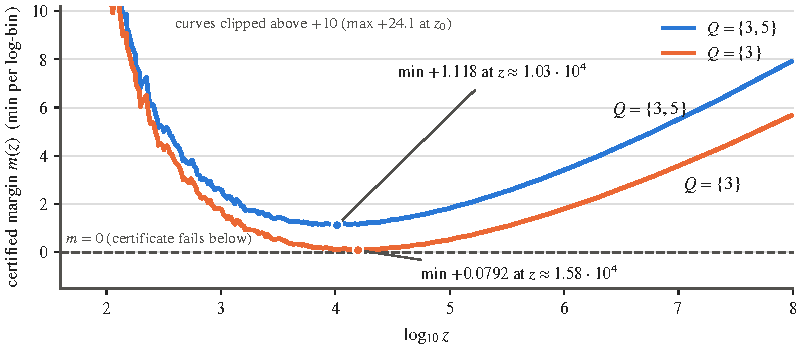
\includegraphics[width=0.8\textwidth]{figs/F1.pdf}
\caption{Certified margin $m_I$ on the finite range, per-cell $K$
(minimum over the cells in each of $400$ logarithmic bins; ball-arithmetic
lower bounds). Blue: $Q=\{3,5\}$, $117\,415$ cells up to $10^8$; orange:
$Q=\{3\}$, same range ($122\,023$ cells up to $10^{10}$ in total).
Both stay above $0$; the dots are the minima of Table~\ref{tab:margins}
(rows I). Nothing in this figure is floating-point only.}
\label{fig:margin}
\end{figure}

\begin{figure}[H]
\centering
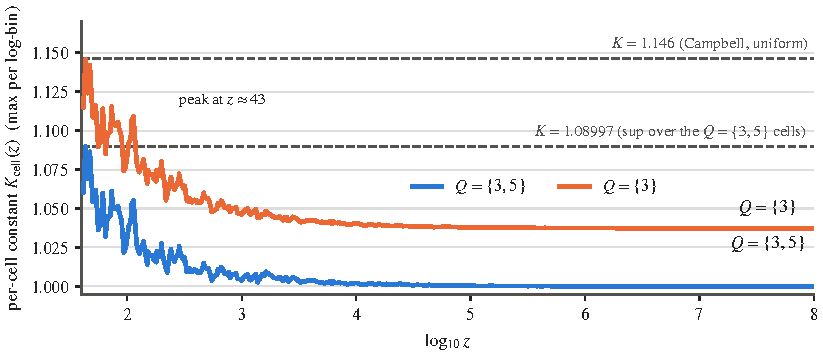
\includegraphics[width=0.8\textwidth]{figs/F2.pdf}
\caption{The certified upper bound $K_I$ for the dimension constant in each
cell (maximum per bin). The per-cell values fall below $1.01$ ($Q=\{3,5\}$)
after $z\approx10^3$ and below $1.04$ ($Q=\{3\}$) after $z\approx2\cdot10^4$, while a uniform constant must
cover the peak near $z\approx43$: Campbell's $1.146$ (dashed) and the
supremum $1.08997$ for $Q=\{3,5\}$ both make the finite range fail
(Section~\ref{subsec:uniform}).}
\label{fig:Kcell}
\end{figure}

\paragraph{Checks by separate implementations}
A separate floating-point implementation, not importing the main code
($147\,347$ geometric cells with $\varepsilon=10^{-4}$, up to exactly
$10^8$), finds the minimum $+1.1188$ on $(10342.337,\,10343.371]$ with no
failing cell. A per-prime evaluation without Jensen bounds (own sieve,
mpmath) agrees with the certificate within $2\cdot10^{-8}$ on $7$ cells,
and on each of them the certificate is the smaller value, as it must be. The identity of Lemma~\ref{lem:identity} was checked exactly
(rational arithmetic) for $859$ odd $N$ and all $d\mid2\cdot7\cdot11\cdot13\cdot17$,
and Lemma~\ref{lem:quad} by brute force for odd $N<1500$ and $60$ values
of $N$ near $30031$, with no violation; these checks cover only small odd $N$.

\subsection{\texorpdfstring{The analytic range $z\ge10^8$}{The analytic range}}

Let $Z$ be an even integer with $Z\ge286$, $t=\log z\ge\log Z$, and
$K_{\mathrm{an}}=K_{\mathrm{an}}(Z)$ from Lemma~\ref{lem:A1}.

\begin{lemma}\label{lem:A2}
For $z\ge Z$, $V(z)\ge c_V/\log^2z$ with
\[
  c_V=e^{-L(Z)}\log^2Z\,e^{-2/\log^2Z-T}.
\]
\end{lemma}

\begin{proof}
$V(z)\ge e^{-L(Z)}\prod_{Z\le p<z}(1-2/p)$, and as in Lemma~\ref{lem:A1},
\[
  -\log\prod_{Z\le p<z}\Bigl(1-\frac2p\Bigr)\le2\log t-2\log\log Z+\frac{2}{\log^2Z}+T.
\]
An upper bound $L_{\mathrm{hi}}$ for $L(Z)$ is used.
\end{proof}

\begin{lemma}\label{lem:A3}
Let $0<\alpha<\log Z$, $\eta=\alpha/t$, $\delta=1-\eta$ and $D=z^s$. Then
\[
  \log2R_4(\cA,D)\le\log(2C_Q)+st-\alpha s+8\log t
  +8\Bigl(B+\frac{1}{2t^2}-\sigma_Q\Bigr)+8(e^\alpha-1),
\]
where $\sigma_{\{3,5\}}=\frac13+\frac15$ (and $\sigma_{\{3\}}=\frac13$).
\end{lemma}

\begin{proof}
By~\eqref{eq:rankin} and $1+x<e^x$,
$R_4\le C_QD^\delta\exp\bigl(8\sum_{p<z,\,p\in\cP}p^{-\delta}\bigr)$. For
$p<z$ write $p^{-\delta}=p^{-1}e^x$ with $x=\eta\log p\in(0,\alpha)$. By
convexity (the chord on $[0,\alpha]$, in place of $e^x<1+xe^x$ used
in~\C), $e^x\le1+x\frac{e^\alpha-1}{\alpha}$, so
$p^{-\delta}\le\frac1p+(e^\alpha-1)\frac{\log p}{pt}$. Summing with (H3)
(upper bound) and (H4) gives
$\sum_{p<z,\,p\in\cP}p^{-\delta}\le\log t+B+\frac{1}{2t^2}-\sigma_Q+(e^\alpha-1)$.
Finally $D^\delta=e^{st-\alpha s}$. A term
$-8(e^\alpha-1)c_Q/t$ with $c_Q=\sum_{q\in Q}\log q/q$ has been dropped;
it enters the margin with a positive sign, so dropping it is conservative.
\end{proof}

\begin{proposition}\label{prop:analytic}
Let $Q=\{3,5\}$, $Z=10^8$,
$k=2+\log K_{\mathrm{an}}$, and fix $s$ and $\alpha$ with $s\ge2k+3$ and
$(A_\pi-s)\log Z>10$. Let $M(t)$ denote the logarithm of the ratio of
$XV(z)F(s,k)$ to $2R_4(\cA,z^s)$. Then $M(t)\ge M_{\mathrm{lo}}(\log Z)$ for
all $t\ge\log Z$, where
\begin{multline*}
  M_{\mathrm{lo}}(t)=A_\pi t+\log c_\pi-\log5+\log(1-16/N)+\log c_V-10\log t
  +\log F(s,k)\\-\log(2C_Q)-st+\alpha s-8(B-\sigma_Q)-\frac{4}{t^2}-8(e^\alpha-1).
\end{multline*}
With the constants of Table~\ref{tab:analytic},
$M_{\mathrm{lo}}(\log Z)\ge+0.654075$ for odd $N$ and $\ge+9.517845$ for
even $N$; hence $S(\cA,z)>0$ for every $N$ with $z\ge10^8$.
\end{proposition}

\begin{proof}
By Lemma~\ref{lem:A1}, Theorem~\ref{thm:local} applies at every $z\ge Z$ with
$k=2+\log K_{\mathrm{an}}$. Write $N=c_\pi e^{A_\pi t}$ and
$X\ge(N-16)/5$ (Lemma~\ref{lem:X}). Lemmas~\ref{lem:A2} and~\ref{lem:A3}
give $M(t)\ge M_{\mathrm{lo}}(t)$; the factor $\log^{-2}z$ from $V$
contributes $-2\log t$ and $R_4$ contributes $-8\log t$. Then
$M_{\mathrm{lo}}(t)=C_0+(A_\pi-s)t-10\log t-4/t^2+\log(1-16/N)$ with a
constant $C_0$, and
\[
  \frac{d}{dt}\Bigl[(A_\pi-s)t-10\log t-\frac{4}{t^2}\Bigr]
  =(A_\pi-s)-\frac{10}{t}+\frac{8}{t^3}>0
\]
whenever $(A_\pi-s)t>10$, which holds for $t\ge\log Z$; the term
$\log(1-16/N)$ is increasing in $t$. Hence $M_{\mathrm{lo}}$ is increasing
on $[\log Z,\infty)$, with no grid. The value $M_{\mathrm{lo}}(\log Z)$ is
evaluated in ball arithmetic.
\end{proof}

\begin{table}[H]
\centering
\caption{Analytic range: constants and certified $M_{\mathrm{lo}}(\log Z)$.
Rows marked ``fixed $K$'' replace $K_{\mathrm{an}}$ by the indicated
constant. Negative values are not certified bounds; they say that the
method fails with these parameters. The values of $s$ and $\alpha$ are
rounded to five decimals; the certified bounds use the double-precision
values printed by \texttt{analytic.py}.}
\label{tab:analytic}
\resizebox{\textwidth}{!}{%
\begin{tabular}{llllllr}
\toprule
$Q$ & $Z$ & $K_{\mathrm{ex}}(Z)\le$ & $K_{\mathrm{an}}$ & $c_V\ge$ & $s$;\ $\alpha$ & $M_{\mathrm{lo}}(\log Z)$\\
\midrule
$\{3,5\}$ & $10^8$    & $1.000061$ & $1.005973$ & $2.068826$ & $14.24820$;\ $0.57719$ & $\mathbf{+0.654075}$\\
$\{3,5\}$, even $N$ & $10^8$ & $1.000061$ & $1.005973$ & $2.068826$ & $14.24815$;\ $0.57719$ & $\mathbf{+9.517845}$\\
$\{3\}$   & $10^8$    & $1.037250$ & $1.043382$ & $1.241296$ & $14.39135$;\ $0.58719$ & $-2.264$\\
$\{3\}$   & $10^9$    & $1.037245$ & $1.042087$ & $1.242838$ & $14.38041$;\ $0.58643$ & $\mathbf{+0.371416}$\\
$\{3\}$   & $10^{10}$ & $1.037243$ & $1.041163$ & $1.243941$ & $14.37186$;\ $0.58583$ & $+3.134105$\\
\midrule
$\{3,5\}$, fixed $K=1.08997$ & $10^8$ & & & & $14.56237$;\ $0.59900$ & $-4.962$\\
$\{3\}$, fixed $K=1.097$ & $10^9$ / $10^{10}$ & & & & & $-3.680$ / $-1.458$\\
$\{3\}$, fixed $K=1.146$ & $10^{10}$ & & & & & $-5.280$\\
\bottomrule
\end{tabular}}
\end{table}

For $Q=\{3,5\}$ and $Z=10^8$ one has $(A_\pi-s)\log Z=32.269$ (odd) and $41.481$ (even), both $>10$, and
$s\ge2k+3$ holds with room to spare. Figure~\ref{fig:analytic} shows
$M_{\mathrm{lo}}$ as a function of $z$.

\begin{figure}[H]
\centering
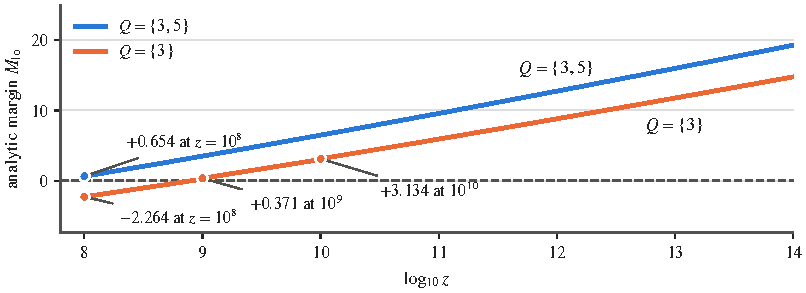
\includegraphics[width=0.85\textwidth]{figs/F3.pdf}
\caption{Analytic range: $M_{\mathrm{lo}}(t)$, $t=\log z$, with the constants
and the $(s,\alpha)$ of Table~\ref{tab:analytic} held fixed (ball-arithmetic
lower endpoints; increasing in $t$ by Proposition~\ref{prop:analytic}). Blue:
$Q=\{3,5\}$, constants of $Z=10^8$. Orange: $Q=\{3\}$, upper envelope of the
curves for $Z=10^8$, $10^9$, $10^{10}$ (lower bounds valid for $z\ge Z$ may
be combined by maximum). The dots are the entries of
Table~\ref{tab:analytic}; the $Q=\{3\}$ curve is negative at $10^8$ and
positive from $10^9$.}
\label{fig:analytic}
\end{figure}

\subsection{Completion of the proof}

Let $N\ge2$. If $N\le N_0$, Corollary~\ref{cor:small} applies. If $N>N_0$
is odd, put $z=(N^2/8)^{1/32}>u_0$; if $N>N_0$ is even, put
$z=(N^2/4)^{1/33}>u_0^{\mathrm{e}}$. If $z\le10^8$, $z$ lies in a cell of
Proposition~\ref{prop:finite} for the parity of $N$ and
Lemma~\ref{lem:margin} gives $S(\cA,z)>0$; if $z\ge10^8$,
Proposition~\ref{prop:analytic} gives $S(\cA,z)>0$. Lemma~\ref{lem:odd}
(odd $N$) or Lemma~\ref{lem:even} (even $N$) then yields $a,b$ with
$N=a+b$ and $\Omega(ab)\le32$. \qed

%% =====================================================================
\section{Remarks}\label{sec:remarks}
%% =====================================================================

\subsection{\texorpdfstring{A second chain with $Q=\{3\}$}{A second chain with Q=\{3\}}}
The theorem also follows from a chain that uses only the constants
of~\cite[\S3]{Campbell2026} ($C_Q=19/6$) and not Section~\ref{subsec:Q35}:
the finite range up to $10^{10}$ with minimal margin $+0.079236$, and the
analytic range from $Z=10^9$ with $+0.371416$ (Tables~\ref{tab:analytic}
and~\ref{tab:margins}); the two ranges overlap. The theorem holds if either
chain is correct; the main chain of this paper is the one with $Q=\{3,5\}$
of Section~\ref{sec:proof}.

\begin{table}[H]
\centering
\caption{Minimal certified margins of the finite range,
$\log(\text{main}/\text{error})$. I: per-cell $K$; E: suffix-maximum
envelope of the per-cell $K$; U: uniform $K$. Negative U values come from a
grid search and mean that the method fails, not certified upper bounds.}
\label{tab:margins}
\resizebox{\textwidth}{!}{%
\begin{tabular}{llrrrrlrrr}
\toprule
$K$ & $Q$ & up to & cells & failing & min.\ margin & cell & $s$ & $\delta$ & $K$\\
\midrule
I & $\{3,5\}$ & $10^8$    & $117\,415$ & $0$ & $\mathbf{+1.118347}$ & $(10342.3367,\,10343.3709]$ & $14.30443$ & $107/128$ & $1.002250$\\
I & $\{3\}$   & $10^{10}$ & $122\,023$ & $0$ & $+0.079236$ & $(15822.3670,\,15823.9492]$ & $14.44136$ & $109/128$ & $1.039801$\\
I, even $N$ & $\{3,5\}$ & $10^8$ & $118\,322$ & $0$ & $+5.024006$ & $(2802.7202,\,2803.0005]$ & $14.34590$ & $102/128$ & $1.005873$\\
E & $\{3,5\}$ & $10^8$    & $117\,415$ & $0$ & $+1.005101$ & same as I & & & $1.005973$\\
E & $\{3\}$   & $10^{10}$ & $122\,023$ & $0$ & $+0.036773$ & same as I & & & $1.041163$\\
U ($K=1.146$)    & $\{3\}$   & $10^8$ & $117\,415$ & $85\,342$ & $-3.405836$ & $z\approx1.18\cdot10^5$ & & & \\
U ($K=1.089970$) & $\{3,5\}$ & $10^8$ & $117\,415$ & $71\,182$ & $-1.671836$ & $z\approx4.29\cdot10^4$ & & & \\
\bottomrule
\end{tabular}}
\end{table}

The envelope variant E, in which $K(z)=\sup_{z''\ge z}K(z'')$, has the
literal form ``for every $z\ge z_a$'' of the lemmas of~\C. It has the same
logical status as the per-cell reading: both rest on
Theorem~\ref{thm:local}.

\subsection{A uniform constant does not suffice}\label{subsec:uniform}
With Campbell's uniform $K=1.146$ and optimised $s,\delta$, the finite range
fails on $85\,342$ of $117\,415$ cells; with $Q=\{3,5\}$ and the uniform
$K=1.089970$ (the supremum over the range) it still fails
(Table~\ref{tab:margins}). So does the analytic range with fixed constants
(Table~\ref{tab:analytic}). The per-cell constant, hence
Theorem~\ref{thm:local}, is essential.

\subsection{\texorpdfstring{Why $\Omega(ab)\le31$ does not follow}{Why 31 does not follow}}
Table~\ref{tab:31} gives exploratory floating-point profiles (a grid of
$60$ points; these are not certified bounds) of the minimum of
$\log(\text{main}/\text{error})$ for the bound $31$.

\begin{table}[H]
\centering
\caption{Exploratory profiles for $\Omega(ab)\le31$ (floating point).}
\label{tab:31}
\resizebox{\textwidth}{!}{%
\begin{tabular}{llrl}
\toprule
case & relation & minimum & where\\
\midrule
odd, $Q=\{3\}$     & $N=\sqrt8\,z^{15.5}$ & $-5.312$ & $z\approx2.03\cdot10^5$; negative on $[534,\,9.9\cdot10^7]$\\
odd, $Q=\{3,5\}$   & same & $-3.947$ & $z\approx5.9\cdot10^4$\\
odd, $Q=\{3,5,7\}$ & same & $-4.167$ & pre-sieving more is worse\\
even, $Q=\{3\}$    & $N=2z^{16}$ & $-0.274$ & negative on $[4659,\,5.6\cdot10^4]$\\
\bottomrule
\end{tabular}}
\end{table}

The deficit of $4$ to $5$ in the logarithm for odd $N$ cannot be closed by
constants; it seems to require a weighted sieve or a better
factor than $F(s,k)$, as suggested in~\cite[\S6]{Campbell2026}.
Figure~\ref{fig:31} shows the profiles for $Q=\{3\}$ and $Q=\{3,5\}$.

\begin{figure}[H]
\centering
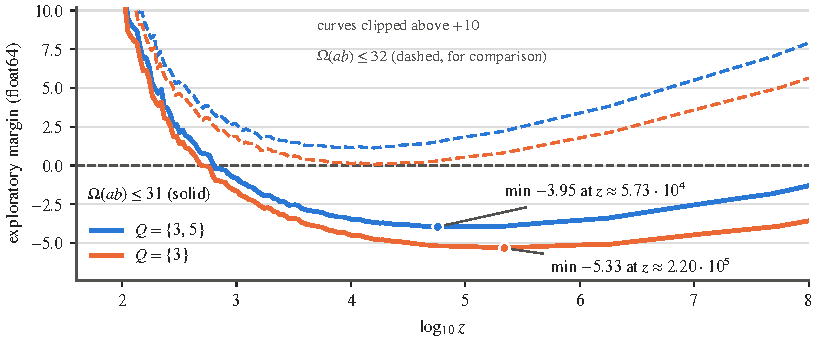
\includegraphics[width=0.8\textwidth]{figs/F4.pdf}
\caption{Why $\Omega(ab)\le31$ does not follow. Solid: exploratory
\emph{floating-point} margin for the bound $31$ ($N=\sqrt8\,z^{15.5}$,
float64, grid of $240$ points, hence slightly below the $60$-point minima of Table~\ref{tab:31}; not a certified bound), negative over most of
the range with minima $-3.95$ ($Q=\{3,5\}$) and $-5.33$ ($Q=\{3\}$). Dashed:
the same computation for the bound $32$, which is positive (certified in
Figure~\ref{fig:margin}).}
\label{fig:31}
\end{figure}

\appendix
\section{Proof of Theorem~\ref{thm:local}}\label{app:sieve}

Throughout this appendix $z$ is fixed, $\cA$, $\cP$, $g$, $X$, $r_d$ are as
in Section~\ref{sec:notation}, and all divisors $d,e,m$ run over divisors
of $P(z)$; they are square-free. The weights $\theta_e$ below are not the
remainders $\rho_\ell$ of~\eqref{eq:rho}, and $Y_0$ is not $Y=N-1$. With
$h$ and $I(U,z)$ as in Section~\ref{subsec:local}, $h(p)>0$ and
$V(z)^{-1}=\prod_{p\mid P(z)}(1+h(p))=\sum_{d\mid P(z)}h(d)$.
Let $D=z^s$ with $s\ge2k+3\ge3$ and $Y_0=\sqrt{D/z}=z^{(s-1)/2}\ge z$.

\paragraph{A.1 Weights}
Let $\psi(d)=\min\{1,\log(Y_0/d)/\log z\}$ for $d<Y_0$ and $\psi(d)=0$ for $d\ge Y_0$;
then $0\le\psi\le1$, $\psi(1)=1$, and $\log d\mapsto \psi(d)$ is
$(1/\log z)$-Lipschitz. Put $J=\sum_d h(d)\psi(d)$, so $1\le J\le V(z)^{-1}$,
$y_d=\psi(d)/J$, and define $\theta_e$ by
\begin{equation}\label{eq:thetay}
  g(e)\theta_e=\mu(e)\sum_{d:\,e\mid d}h(d)y_d .
\end{equation}
Then $\theta_1=\sum_dh(d)y_d=1$ and $\theta_e=0$ for $e\ge Y_0$. Moreover
$|\theta_e|\le1$: since $h(e)/g(e)=\prod_{p\mid e}(1+h(p))=\sum_{t\mid e}h(t)$,
\[
  |\theta_e|=\frac1J\sum_{t\mid e}\ \sum_{f:\,(f,e)=1}h(t)h(f)\,\psi(ef)
  \le\frac1J\sum_{t\mid e}\ \sum_{f:\,(f,e)=1}h(tf)\,\psi(tf)\le1,
\]
because $\psi$ is non-increasing, $tf\le ef$, and distinct pairs $(t,f)$ give
distinct $d=tf$. M\"obius inversion of~\eqref{eq:thetay} gives
\begin{equation}\label{eq:Fe}
  \sum_{m:\,e\mid m}g(m)\theta_m=\mu(e)h(e)y_e .
\end{equation}

\paragraph{A.2 The lower bound sieve}
For every integer $a$,
\[
  \mathbf 1_{(a,P(z))=1}\ \ge\ \Bigl(1-\sum_{p\mid(a,P(z))}1\Bigr)
  \Bigl(\sum_{d\mid(a,P(z))}\theta_d\Bigr)^2 ,
\]
since both sides equal $1$ if $(a,P(z))=1$, and otherwise the first factor
is $\le0$. Summing over $n$ gives $S(\cA,z)\ge\sum_d\lambda_d|\cA_d|$ with
\[
  \lambda_d=\lambda^+_d-\sum_{p\mid d}\bigl(\lambda^+_d+\lambda^+_{d/p}\bigr),
  \qquad
  \lambda^+_d=\sum_{[d_1,d_2]=d}\theta_{d_1}\theta_{d_2},
\]
hence $S(\cA,z)\ge XV(D,z)-\sum_d|\lambda_d||r_d|$ with
$V(D,z)=\sum_d\lambda_dg(d)$.

\paragraph{A.3 The main term}
Since $g([d_1,d_2])=g(d_1)g(d_2)/g((d_1,d_2))$ and
$1/g(m)=\sum_{e\mid m}1/h(e)$, \eqref{eq:Fe} gives
$\sum_{d_1,d_2}\theta_{d_1}\theta_{d_2}g([d_1,d_2])=\sum_eh(e)y_e^2$. For a
fixed $p$, write $d_i=p^{\varepsilon_i}d_i'$ with $p\nmid d_i'$; then
$g([p,d_1,d_2])=g(p)g([d_1',d_2'])$, and the same diagonalisation over
$p\nmid e$, with $\sum_{e\mid m,\,p\nmid m}g(m)(\theta_m+\theta_{pm})
=\mu(e)h(e)(y_e-y_{pe})$ by~\eqref{eq:Fe}, gives
\begin{equation}\label{eq:VDz}
  V(D,z)=\sum_dh(d)y_d^2-\sum_{p\nmid d}g(p)h(d)\bigl(y_d-y_{pd}\bigr)^2 .
\end{equation}
This is~\cite[(2.3)]{Blight2010}. Using $g(p)\le h(p)$ and putting $m=pd$,
\[
  V(D,z)\ge\sum_mh(m)\Bigl(y_m^2-\sum_{p\mid m}(y_{m/p}-y_m)^2\Bigr).
\]
If $m\le Y_0/z$, then $\psi(m/p)=\psi(m)=1$; if $m\ge Yz$, then $m/p>Y_0$ and
$\psi(m/p)=\psi(m)=0$; in both cases the inner sum vanishes. If $Y_0/z<m<Yz$, the
Lipschitz property gives
$\sum_{p\mid m}(y_{m/p}-y_m)^2\le J^{-2}\sum_{p\mid m}(\log p/\log z)^2
\le J^{-2}\log m/\log z$, as $p<z$. Dropping $y_m^2\ge0$ on this range,
\[
  J^2V(D,z)\ \ge\sum_{m\le Y_0/z}h(m)-\frac{\log(Yz)}{\log z}\sum_{m>Y_0/z}h(m)
  \ \ge\ V(z)^{-1}-\frac{\log(Yz^2)}{\log z}\,I(Y_0/z,z),
\]
and $\log(Yz^2)/\log z=(s+3)/2$. (In~\cite[\S2.3]{Blight2010} the
normalisation is written $J=\sum_{d\le Y_0}h(d)$; the argument only needs
$\theta_1=1$ and $J\le V(z)^{-1}$, which hold for the $J$ above.)

\paragraph{A.4 The remainder}
For $d$ with $\omega(d)=\omega\ge1$, $|\lambda^+_d|\le3^{\omega}$ because
$|\theta|\le1$, so $|\lambda_d|\le(\omega-1)3^{\omega}+\omega3^{\omega-1}
=3^{\omega-1}(4\omega-3)\le1.38\cdot4^{\omega}\le2\tau_4(d)$, and
$\lambda_1=1$. If $\lambda_d\ne0$, then $d\mid p\,d_1d_2$ with $p<z$ and
$d_1,d_2<Y_0$, so $d<zY_0^2=D$. Hence $\sum_d|\lambda_d||r_d|\le2R_4(\cA,D)$,
using $r_1=0$.

\paragraph{A.5 Conclusion}
Apply Proposition~\ref{prop:rankinK} with $U=Y_0/z$, so that
$u=\log U/\log z=(s-3)/2\ge k$:
\[
  \frac{s+3}{2}\,I(Y_0/z,z)V(z)\le\frac{s+3}{2e^{k}}
  \Bigl(\frac{2ek}{s-3}\Bigr)^{(s-3)/2}=1-F(s,k).
\]
If $F(s,k)\le0$, the claim $S(\cA,z)\ge XV(z)F(s,k)-2R_4(\cA,D)$ is
trivial, since $S(\cA,z)\ge0$. If $F(s,k)>0$, A.3 gives
$J^2V(D,z)V(z)\ge F(s,k)>0$, and $J\le V(z)^{-1}$ gives
$V(D,z)\ge F(s,k)/(J^2V(z))\ge V(z)F(s,k)$. By A.2 and A.4,
$S(\cA,z)\ge XV(z)F(s,k)-2R_4(\cA,D)$. The dimension condition was used
only in Proposition~\ref{prop:rankinK}, at the level $z$. \qed

\paragraph{Numerical check}
The script \texttt{test\_local\_sieve.py} in the directory
\texttt{certificate/local\_sieve} of the repository (output file
\texttt{out\_test\_local\_sieve.txt}) tests these steps for $300$ random densities and for the sequences $\cA$ of
this paper with $Q=\{3\}$ and $\{3,5\}$, odd $N$ and even $N$ in
$[41,400)$ together with four larger values up to $9999$, $z\le18$ and
$s\in[2,24]$ ($29\,040$ cases), with no violation. With the weights
$\psi(d)$ replaced by rational approximations, the identity~\eqref{eq:VDz},
$\theta_1=1$, $|\theta_e|\le1$, $|\lambda_d|\le2\tau_4(d)$, the support
$d<D$ and the inequality $S(\cA,z)\ge\sum_d\lambda_d|\cA_d|$ are checked in
exact rational arithmetic; the bound of A.3, Proposition~\ref{prop:rankinK}
and the conclusion $S(\cA,z)\ge XV(z)F(s,k)-2R_4(\cA,D)$ (with $\kappa=2$
and the smallest $K$ allowed at this $z$) are checked in floating point
with a relative tolerance of $10^{-9}$, the last two in the $20\,328$ cases
with $s\ge2k+3$, of which $11\,181$ have $F(s,k)>0$. The test checks the
algebra; it is not part of the proof.

%% =====================================================================
\section*{Use of AI tools in the research}
%% =====================================================================

Claude Opus~5.5 (Anthropic), used through the Claude Code agent
environment, took part in the research as follows. It first proposed and
derived the three reductions of Section~\ref{sec:reductions}; the
adaptation to $Q=\{3,5\}$ (Lemmas~\ref{lem:identity}--\ref{lem:X}); the
reduction of the per-cell constant to finitely many candidates
(Lemma~\ref{lem:Kcell}); Lemmas~\ref{lem:A1}--\ref{lem:A3} and the
monotonicity argument of Proposition~\ref{prop:analytic}; the analysis of
the reading of~\eqref{eq:dim} in Section~\ref{subsec:local}, including
the literature search behind Remark~\ref{rem:evidence};
Proposition~\ref{prop:rankinK}; the proof of Theorem~\ref{thm:local} in
Appendix~\ref{app:sieve}, including the case distinction on the sign of
$F$, which was found by a numerical test of each step
(script \texttt{test\_local\_sieve.py}); and the
treatment of even $N$ (Lemma~\ref{lem:even}). It wrote all the code of the certificate
(prime sieve, ball-arithmetic bounds, cell cover, analytic range) and the
scripts that draw Figures~\ref{fig:margin}--\ref{fig:31} directly from
the certificate outputs. The checks described under ``Checks by separate
implementations'' were written by separate instances of the same tool,
which did not import the main code; their agreement is internal
consistency, not independent human verification. The checks that do not
rely on AI-written arithmetic are the comparison of prime counts and block
sums with primesieve~12.17 and of $\pi(10^k)$, $k\le10$, with known
values. The author checked every proof by hand; the certificate is
deterministic, and re-running the published code reproduces all
certificate outputs bit for bit except the wall-clock timing lines
(Code availability statement).

%% =====================================================================
\section*{Code availability statement}
%% =====================================================================

\begin{sloppypar}
Code and certificate outputs are available at
\url{https://github.com/giovanedms/goldbach-omega32} (Zenodo DOI to be assigned). The repository
contains: \texttt{primes\_blocks.py} (exact counts
and sums of primes per block up to $10^{10}$), \texttt{check\_blocks.py}
(comparison with primesieve), \texttt{rlib.py} (ball arithmetic),
\texttt{run\_cover.py} (finite range), \texttt{analytic.py} (analytic
range), \texttt{test\_local.py} (brute force of the local lemmas),
\texttt{test\_local\_sieve.py} (numerical test of the algebra of Appendix~\ref{app:sieve}), and
their outputs. Environment: Python 3.14.4, python-flint 0.9.0, numpy 2.5.4,
mpmath 1.3.0, primesieve 12.17; no GPU. The main finite cover
(\texttt{run\_cover.py 3,5 1e8 interval}) runs in about $40$\,s; the even
case is the same command with the environment variable
\texttt{GB\_PARITY=even} (about $70$\,s), followed by
\texttt{analytic.py 3,5 1e8}.
Campbell's scripts~\cite{CampbellRepo} were re-run at commit
\texttt{2755a58b6eb1\ldots} and reproduce the versioned output byte for
byte. SHA-256 of the main files:
\end{sloppypar}

\begingroup\fontsize{7}{8.5}\selectfont
\begin{verbatim}
7e8eb38ada4507a5599631cd2511db23d1d81d9f501a29d8c5da5e8163b1566c  out_cover_Q35_interval.txt
c1d879bed47e8b3ce647e62bb1b9657529ea7d96f051cb34b7745a221240bad8  out_cover_Q35_interval_even.txt
9d4dba8e248b89e284dbb3e57e16f2474b03b72bbb8725c30db6fa90e677259b  out_cover_Q3_interval.txt
b0d1624d1eb576a1ab9066db8abb06c54954598467d58a5e49382d23808bb0fa  out_analytic.txt
ca269994cbf54fbb438422fd18c38bd1aad9e2f10dce3f940375fc64a3cdbe91  out_analytic_even.txt
f44c4b01fddeb9b4b6e933fe291daedf3b84247dce68b24abe6490bce1c44b9a  rlib.py
0acb487e5dd3bffef14ce2c5a9b358d41cf19b06e53015349af49c713f236c5a  run_cover.py
84483ca099c5029ab112e445ab48e26542f2cf9af4f2770745d56628c7732356  analytic.py
4e901d77dfc171bce886f9924b9d8a0e59eb26b0b517a7ec53198cb7c552d86f  primes_blocks.py
f87ba8e8369686cc06c1db203828e79f5f70a8b90f0bf1cdf20fc91b858365f8  test_local_sieve.py
5e21da3a192ba96e952c4e29602894e695703b6a7c49a7526e93fd5c97457ee1  out_test_local_sieve.txt
\end{verbatim}
\endgroup

\section*{Acknowledgements}
The author thanks Peter J.\ Campbell for making his verification scripts
publicly available under the MIT licence, and for the list of refinements
in~\cite[\S6]{Campbell2026}, three of which are used here.

\section*{Declaration of generative AI and AI-assisted technologies in the manuscript preparation process}

During the preparation of this work the author used Claude Opus~5.5
(Anthropic), through the Claude Code agent environment, to draft the
manuscript from a technical dossier of the proofs, and to organise and
edit the text. The use of the same tool in the research itself is
described in the section ``Use of AI tools in the research'' above.
After using this tool, the author reviewed and edited the content as
needed, checked the proofs by hand, and takes full responsibility for the
content of the published article.

\section*{Funding}
This research did not receive any specific grant from funding agencies in the public,
commercial, or not-for-profit sectors.

\section*{Declaration of competing interest}
The author declares no competing interests.


\bibliographystyle{elsarticle-num}
\bibliography{refs}

\end{document}
